\documentclass[9pt]{beamer}
\usetheme{Madrid}
\usecolortheme{default}
\usepackage{amsmath, amssymb, amsthm}
\usepackage{tikz}
\usetikzlibrary{shapes, arrows, positioning}

% Title, Subtitle, Author, and Institution details
\title[Query Embeddings in Text-to-SQL]{Analyzing Query Embedding Spaces in RAG-Based Text-to-SQL Systems Using PCA and SVM}
\subtitle{Bridging Mathematics and AI}
\author[Akanksha Parab]{Akanksha Parab}
\institute[St. Xavier's College]{
    TYBSc Mathematics (Major) | Statistics (Minor)\\
    St. Xavier's College, Mumbai\\
    \medskip
    \small Summer Internship Research Presentation
}
\date[August 24, 2026]{August 24, 2026}

\begin{document}

% === Slide 1: Title Frame ===
\begin{frame}
    \titlepage
\end{frame}
% SCRIPT FOR SLIDE 1:
% "Good afternoon, everyone. Thank you for being here. My name is Akanksha Parab, and I am currently in my final year pursuing my BSc in Mathematics with a minor in Statistics here at St. Xavier’s.
%
% Today, I want to talk to you about something that sits right at the intersection of our daily mathematics lectures and the rapidly evolving world of Artificial Intelligence. Over the summer, I did my internship at an AI services startup, where I focused on a research project titled 'Analyzing Query Embedding Spaces in RAG-Based Text-to-SQL Systems Using PCA and SVM.'
%
% Now, that title might sound like a mouthful of computer science jargon, but at its heart, this research is driven entirely by the mathematical concepts we study in our classrooms. If you have ever sat in a Linear Algebra lecture wondering why we study vector spaces, dimension, or eigenvalues, or in a Real Analysis class wondering about metric spaces and distance, this presentation is for you.
%
% We will see how these exact concepts are used to help database systems understand human language. Specifically, we will look at how we convert English questions into high-dimensional geometric coordinates, use Principal Component Analysis to find the 'true' shape of that data, and use Support Vector Machines to classify query complexity so we can route queries to the most cost-effective AI models.
%
% My goal today is to show you that mathematics is not just abstract theory written on a blackboard; it is the concrete architecture of modern AI. Let's start by looking at the core problem my research addresses."

% === Slide 2: The Core Problem ===
\begin{frame}{The Core Problem: Enterprise Query Routing}
    \begin{columns}
        \begin{column}{0.55\textwidth}
            \textbf{The Challenge in Text-to-SQL RAG:}
            \begin{itemize}
                \item \textbf{Text-to-SQL:} Translating natural language queries $q \in Q$ into executable SQL code.
                \item \textbf{Resource Trade-off:} Large Language Models (LLMs) are accurate but expensive and slow. Small models (SLMs) are fast and cheap but fail on complex schema joins.
            \end{itemize}
            \vspace{0.45cm}
            \textbf{Mathematical Goal:}
            Find a routing function $R: Q \rightarrow \{M_{\text{small}}, M_{\text{large}}\}$ that minimizes inference cost and latency $C(R(q))$ subject to a target accuracy threshold $\alpha$:
            \[
            \min_{R} \mathbb{E}[C(R(q))] \quad \text{subject to} \quad \text{Acc}(R(q)) \ge \alpha
            \]
        \end{column}
        
        \begin{column}{0.45\textwidth}
            \centering
            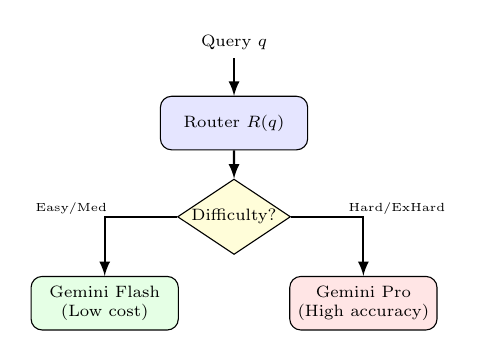
\begin{tikzpicture}[scale=0.85, transform shape,
                node distance=1.2cm,
                box/.style={draw, rectangle, rounded corners, minimum width=2.2cm, minimum height=0.8cm, fill=blue!10, align=center, font=\scriptsize},
                decision/.style={draw, diamond, aspect=1.5, fill=yellow!15, align=center, font=\scriptsize, inner sep=0.5pt},
                arrow/.style={-latex, thick}
            ]
                % Nodes
                \node (input) [align=center] {\scriptsize Query $q$};
                \node (router) [box, below of=input] {Router $R(q)$};
                \node (eval) [decision, below of=router, node distance=1.4cm] {Difficulty?};
                \node (small) [box, below left=0.6cm and 0.4cm of eval, fill=green!10] {Gemini Flash \\ (Low cost)};
                \node (large) [box, below right=0.6cm and 0.4cm of eval, fill=red!10] {Gemini Pro \\ (High accuracy)};

                % Arrows
                \draw [arrow] (input) -- (router);
                \draw [arrow] (router) -- (eval);
                \draw [arrow] (eval) -| node[above, xshift=-0.5cm, yshift=-0.1cm] {\tiny Easy/Med} (small);
                \draw [arrow] (eval) -| node[above, xshift=0.5cm, yshift=-0.1cm] {\tiny Hard/ExHard} (large);
            \end{tikzpicture}
        \end{column}
    \end{columns}
\end{frame}
% SCRIPT FOR SLIDE 2:
% "Now let's delve into the actual problem my summer research addressed. In modern enterprise systems, we often build Text-to-SQL pipelines—systems that take a plain English question from a user, translate it into database SQL code, query the database, and return the answer.
%
% But here is the catch: not all questions are created equal. If a user asks, 'What is the average price of books?', that is a simple query requiring a single table select. But if they ask, 'Show the top three authors who have written books in more than five genres, ordered by their average publication rating,' that query requires complex inner joins, aggregations, and subqueries.
%
% Historically, companies route all queries to the most powerful model, like Gemini Pro or GPT-4. This is highly accurate, but it is also incredibly slow and expensive. Alternatively, routing everything to a smaller, cheaper model like Gemini Flash saves money but fails on the complex, multi-join queries.
%
% As mathematicians, we can formalize this trade-off as a constrained optimization problem. Let Q be the set of all possible natural language queries. We want to find a mapping—a routing function R—that routes a query q to either a small model M_small or a large model M_large.
%
% Our mathematical objective is to minimize the expected cost and latency C(R(q)) of these runs, subject to the constraint that our overall pipeline accuracy remains above some target threshold \alpha.
%
% The challenge is: how do we build this routing function R(q) if q is just a string of English words? We cannot calculate functions or distances on text directly. We must first map the text into a mathematical space where we can run calculations. This brings us to vector space embeddings."

% === Slide 3: High-Dimensional Vector Spaces ===
\begin{frame}{High-Dimensional Vector Spaces (\(\mathbb{R}^{768}\))}
    \begin{columns}
        \begin{column}{0.55\textwidth}
            \textbf{Text Vectorization}
            \begin{itemize}
                \item We use a pre-trained \textbf{Sentence Transformer} model currently running on Sumvec's live platform.
                \item The model maps a natural language query to a dense vector:
                \[
                f: \text{Query} \rightarrow \mathbf{v} \in \mathbb{R}^{768}
                \]
                \item Each of the 768 numbers is a coordinate representing a latent semantic feature.
            \end{itemize}
            \vspace{0.45cm}
            \textbf{Cosine Similarity}
            To measure semantic similarity, we compute the angle $\theta$ between vectors using the inner product:
            \[
            \cos(\theta) = \frac{\mathbf{u} \cdot \mathbf{v}}{\|\mathbf{u}\|_2 \|\mathbf{v}\|_2}
            \]
        \end{column}
        
        \begin{column}{0.45\textwidth}
            \centering
            \textbf{\small Semantic Proximity in \(\mathbb{R}^2\)}
            \vspace{0.3cm}
            
            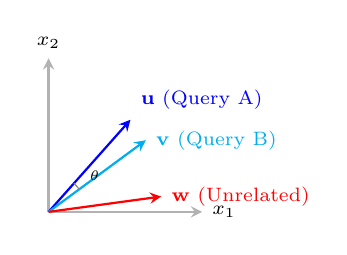
\begin{tikzpicture}[scale=1.3, >=stealth, thick]
                \draw[->, gray!60] (0,0) -- (1.5,0) node[right, black] {\scriptsize $x_1$};
                \draw[->, gray!60] (0,0) -- (0,1.5) node[above, black] {\scriptsize $x_2$};
                
                \draw[->, blue] (0,0) -- (0.8, 0.9) node[above right] {\scriptsize $\mathbf{u}$ (Query A)};
                \draw[->, cyan] (0,0) -- (0.95, 0.7) node[right] {\scriptsize $\mathbf{v}$ (Query B)};
                \draw[->, red] (0,0) -- (1.1, 0.15) node[right] {\scriptsize $\mathbf{w}$ (Unrelated)};
                
                \draw[gray, thin] (0.3,0.22) arc (36:48:0.38);
                \node at (0.45, 0.35) {\tiny $\theta$};
            \end{tikzpicture}
        \end{column}
    \end{columns}
\end{frame}
% SCRIPT FOR SLIDE 3:
% "To build a router that classifies queries, we must first convert human language into a format that computers can run calculations on. In our applied AI system, we use a pre-trained Sentence Transformer model. This is the exact same model running on Sumvec's live production platform, ensuring our research matches real-world traffic.
%
% When a user enters a query, the model acts as a function, mapping the text into a 768-dimensional real vector space, \mathbb{R}^{768}. Instead of a 2D coordinate like (x, y), a query becomes a list of 768 coordinates. Each coordinate represents a semantic feature learned by the model during training.
%
% The core mathematical idea is that sentences with similar meanings will point in similar directions in this space. To measure this closeness, we use cosine similarity, which computes the cosine of the angle \theta between two vectors.
%
% As you can see in the diagram on the right, if we project this space to 2D: Query A, 'Select all employees,' and Query B, 'List the staff members,' point in nearly the same direction with a tiny angle \theta between them, yielding a cosine similarity close to 1. Meanwhile, an unrelated query like 'What is the capital of France?' points in a completely different direction, making it nearly orthogonal, with a similarity close to 0."

% === Slide 4: Vector Norms and Normalization ===
\begin{frame}{Vector Norms and Geometric Normalization}
    \begin{columns}
        \begin{column}{0.55\textwidth}
            \textbf{Similarity Retrieval}
            \begin{itemize}
                \item Longer sentences naturally produce vectors with larger magnitudes.
                \item To compare queries purely by meaning, we must eliminate the effect of length and isolate vector \textbf{direction}.
            \end{itemize}
            \vspace{0.15cm}
            \textbf{Vector Norms}
            For a vector $\mathbf{x} \in \mathbb{R}^{768}$, its Euclidean ($L_2$) norm is:
            \[
            \|\mathbf{x}\|_2 = \sqrt{\sum_{i=1}^{768} x_i^2}
            \]
            We normalize the vector to unit length ($1.0$):
            \[
            \hat{\mathbf{x}} = \frac{\mathbf{x}}{\|\mathbf{x}\|_2} \quad \implies \quad \|\hat{\mathbf{x}}\|_2 = 1
            \]
            This simplifies cosine similarity to a simple dot product: $\hat{\mathbf{u}} \cdot \hat{\mathbf{v}}$.
        \end{column}
        
        \begin{column}{0.45\textwidth}
            \centering
            \textbf{\small Projection onto the Unit Circle}
            \vspace{0.2cm}
            
            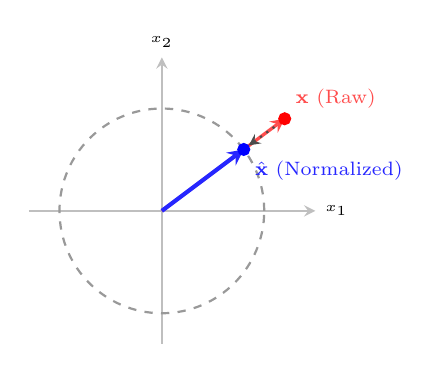
\begin{tikzpicture}[scale=1.3, >=stealth, thick]
                \draw[->, gray!50] (-1.3,0) -- (1.5,0) node[right, black] {\tiny $x_1$};
                \draw[->, gray!50] (0,-1.3) -- (0,1.5) node[above, black] {\tiny $x_2$};
                \draw[dashed, gray!80] (0,0) circle (1.0);
                
                \draw[->, red!70, line width=1.2pt] (0,0) -- (1.2, 0.9) node[above right] {\scriptsize $\mathbf{x}$ (Raw)};
                \draw[->, blue!85, line width=1.5pt] (0,0) -- (0.8, 0.6) node[below right] {\scriptsize $\hat{\mathbf{x}}$ (Normalized)};
                \draw[->, dotted, black!70, thick] (1.1,0.82) -- (0.85,0.64);
                
                \filldraw[blue] (0.8,0.6) circle (1.5pt);
                \filldraw[red] (1.2,0.9) circle (1.5pt);
            \end{tikzpicture}
        \end{column}
    \end{columns}
\end{frame}
% SCRIPT FOR SLIDE 4:
% "In applied AI, we want to match queries based on their semantic direction. However, longer sentences naturally contain more words, which can skew the length, or magnitude, of their vectors. If we don't account for this, the system might think two queries are different simply because one has more words than the other.
%
% To prevent this, we perform unit normalization.
%
% Mathematically, we define the length of a vector using the Euclidean norm, or L_2 norm. This is the square root of the sum of the squared coordinates. To isolate the direction, we divide our raw vector \mathbf{x} by its norm, producing a normalized unit vector \hat{\mathbf{x}} with a magnitude of exactly 1.0.
%
% You can see this projection in the 2D diagram on the right. The dashed circle represents the boundary where the distance from the origin is exactly 1.0. The red arrow is our raw vector, which extends past this boundary. By dividing by its norm, we scale it down along its path until its tip sits exactly on the circle, resulting in the blue vector \hat{\mathbf{x}}.
%
% The great mathematical advantage of this is that when all vectors have a length of 1.0, the denominator in our cosine similarity formula simplifies to 1 \times 1 = 1. This means similarity can be calculated using a simple dot product, which is computationally very fast.
%
% Now let's look at how we validate our query difficulty labels."

% === Slide 5: Data Distribution and Class Imbalance ===
\begin{frame}{Data Distribution and Class Imbalance}
    \begin{columns}[t]
        \begin{column}{0.5\textwidth}
            \textbf{Dataset Comparison:}
            \vspace{0.1cm}
            \begin{table}
                \centering
                \scriptsize
                \begin{tabular}{lcc}
                    \hline
                    \textbf{Metric} & \textbf{Spider} & \textbf{Pinecone} \\ \hline
                    Dataset Type & Benchmark & Production \\
                    Observations & 10,000 & 11,435 \\
                    Embedding Dim & 384D & 768D \\
                    Complexity & Static & Live Traffic \\ \hline
                \end{tabular}
            \end{table}
        \end{column}
        
        \begin{column}{0.5\textwidth}
            \textbf{Complexity Distribution:}
            \vspace{0.1cm}
            \begin{table}
                \centering
                \scriptsize
                \begin{tabular}{llc}
                    \hline
                    \textbf{Difficulty} & \textbf{Criteria} & \textbf{Empirical \%} \\ \hline
                    Easy & $S = 0$ & $\approx 25\%$ \\
                    Medium & $S = 1$ & $\approx 33\%$ \\
                    Hard & $S \in \{2, 3\}$ & $\approx 27\%$ \\
                    Extra Hard & $S \ge 4$ & $\approx 15\%$ \\ \hline
                \end{tabular}
            \end{table}
        \end{column}
    \end{columns}
    
    \vspace{0.45cm}
    \begin{columns}[t]
        \begin{column}{0.5\textwidth}
            \textbf{Heuristic Labeling ($S$):}
            Based on SQL keyword counts:
            \begin{itemize}
                \scriptsize
                \item JOINs, GROUP BYs, Subqueries
                \item $S$ score mapping to labels
            \end{itemize}
        \end{column}
        
        \begin{column}{0.5\textwidth}
            \textbf{Statistical Imbalance:}
            In both academic benchmark and live production traffic, the \textbf{Extra Hard} class represents only $\approx 15\%$ of the total data. 
            \begin{itemize}
                \scriptsize
                \item Models naturally over-predict the majority classes.
                \item Requires balancing class weights in optimization.
            \end{itemize}
        \end{column}
    \end{columns}
\end{frame}
% SCRIPT FOR SLIDE 5:
% "After vectorizing our queries, the next step is labeling them by complexity. In our research, we work with two distinct datasets. The first is the academic benchmark dataset, Spider, containing 10,000 query pairs mapped to 384-dimensional vectors. The second is the live production database on Pinecone, which contains over 11,000 queries mapped to 768 dimensions.
%
% To classify them, we use a heuristic parser that scores each query based on its SQL structure—assigning points for keywords like JOINs, GROUP BYs, and nested subqueries. This score groups our queries into four difficulty categories: Easy, Medium, Hard, and Extra Hard.
%
% However, looking at the distribution, we observe a classical statistics problem: class imbalance. In both the academic dataset and live production traffic, Easy and Medium queries dominate the dataset, while 'Extra Hard' queries represent a small minority of only 15%.
%
% For our routing classifier, this imbalance is dangerous. If a machine learning model is trained on imbalanced data, it will naturally try to achieve high accuracy by predicting the majority classes and ignoring the minority 'Extra Hard' queries. Since misrouting an 'Extra Hard' query causes a pipeline failure, we must correct this imbalance later.
%
% But first, we face a major geometric obstacle. With 768 dimensions in production, how do we handle the vast empty space where our data lies? Let's discuss the curse of dimensionality."

% === Slide 6: The Curse of Dimensionality ===
\begin{frame}{The Curse of Dimensionality \& Redundancy}
    \begin{columns}
        \begin{column}{0.55\textwidth}
            \textbf{Curse of Dimensionality:}
            \begin{itemize}
                \item \textbf{Volume Expansion:} The volume of a hypercube scales exponentially ($s^d$).
                \item \textbf{Data Sparsity:} In high dimensions ($d=768$), data points become extremely isolated.
                \item \textbf{Distance Convergence:} Distances between random points converge to a constant value, making neighborhoods unstable.
            \end{itemize}
               \vspace{0.45cm}
            \textbf{Semantic Noise \& Redundancy:}
            \begin{itemize}
                \item A 10\% loss in variance represents \textbf{"noise"}—variations in punctuation or phrasing that do not change query intent.
                \item Real information lies on a much lower-dimensional manifold.
            \end{itemize}
        \end{column}
        
        \begin{column}{0.45\textwidth}
            \centering
            \textbf{\small Spatial Sparsity ($2^d$)}
            \vspace{0.2cm}
            
            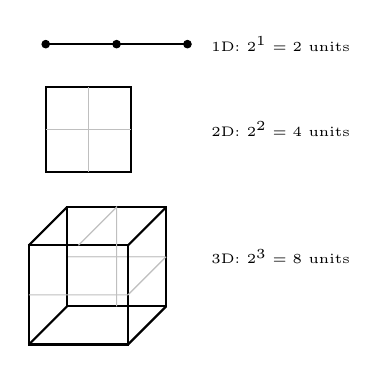
\begin{tikzpicture}[scale=0.9, >=stealth]
                \draw[thick] (0,3) -- (2,3);
                \filldraw (0,3) circle (1.5pt);
                \filldraw (1,3) circle (1.5pt);
                \filldraw (2,3) circle (1.5pt);
                \node[right] at (2.2,3) {\tiny 1D: $2^1=2$ units};
                
                \draw[thick] (0,1.2) rectangle (1.2, 2.4);
                \draw[gray!50, thin] (0.6,1.2) -- (0.6,2.4);
                \draw[gray!50, thin] (0,1.8) -- (1.2,1.8);
                \node[right] at (2.2, 1.8) {\tiny 2D: $2^2=4$ units};
                
                \begin{scope}[shift={(0.3,-0.7)}, scale=0.7]
                    \draw[gray!40, thin] (0,1,0) -- (2,1,0) -- (2,1,2);
                    \draw[thick] (0,0,0) -- (2,0,0) -- (2,2,0) -- (0,2,0) -- cycle;
                    \draw[thick] (0,0,2) -- (2,0,2) -- (2,2,2) -- (0,2,2) -- cycle;
                    \draw[thick] (0,0,0) -- (0,0,2);
                    \draw[thick] (2,0,0) -- (2,0,2);
                    \draw[thick] (2,2,0) -- (2,2,2);
                    \draw[thick] (0,2,0) -- (0,2,2);
                    \draw[gray!50, thin] (1,0,0) -- (1,2,0) -- (1,2,2);
                    \draw[gray!50, thin] (0,1,2) -- (2,1,2) -- (2,1,0);
                \end{scope}
                \node[right] at (2.2, 0) {\tiny 3D: $2^3=8$ units};
            \end{tikzpicture}
        \end{column}
    \end{columns}
\end{frame}
% SCRIPT FOR SLIDE 6:
% "Now, why is working in a 768-dimensional space a problem? It comes down to a fundamental mathematical concept called the Curse of Dimensionality.
%
% As we increase the dimension d of a space, its volume grows exponentially. If we divide a 1-dimensional line segment in half, we get 2 sections. For a 2D square, we get 4 quadrants. For a 3D cube, we get 8 octants. If we scale this to a 768-dimensional hypercube, dividing it along each axis gives us 2^{768} sub-regions.
%
% Because this volume is so massive, our 11,000 query vectors are incredibly isolated from one another. They float in a vast, empty space where distance metrics become unstable—meaning the distance between any two queries starts to look nearly identical.
%
% But here is the key semantic insight: natural language is structured and highly redundant. A query vector doesn't need all 768 coordinates to express its meaning. In fact, we discovered that we can discard 10% of the variance in our dataset because it is mostly 'noise.' This noise represents tiny variations in punctuation, capitalization, or spelling that do not change the query's actual database intent.
%
% By removing this noise, we can contract our space and find a much tighter, lower-dimensional coordinate system. To do this, we use Principal Component Analysis."

% === Slide 7: Principal Component Analysis ===
\begin{frame}{Principal Component Analysis (PCA)}
    \begin{columns}
        \begin{column}{0.5\textwidth}
            \textbf{PCA as a Change of Basis:}
            A vector can be represented using different bases. 
            \begin{itemize}
                \item PCA finds the \textbf{best orthonormal basis} for the data.
                \item The first basis vector points in the direction of maximum variance (spread).
                \item Each subsequent basis vector is orthogonal to the previous ones.
            \end{itemize}
            \vspace{0.45cm}
            \textbf{Production Insights (768D):}
            \begin{itemize}
                \item Retaining \textbf{90\% variance} requires only \textbf{220 components}.
                \item Represents a \textbf{71\% dimensionality reduction} in production.
            \end{itemize}
        \end{column}
        
        \begin{column}{0.5\textwidth}
            \centering
            \textbf{\small Cumulative Explained Variance}
            \vspace{0.1cm}
            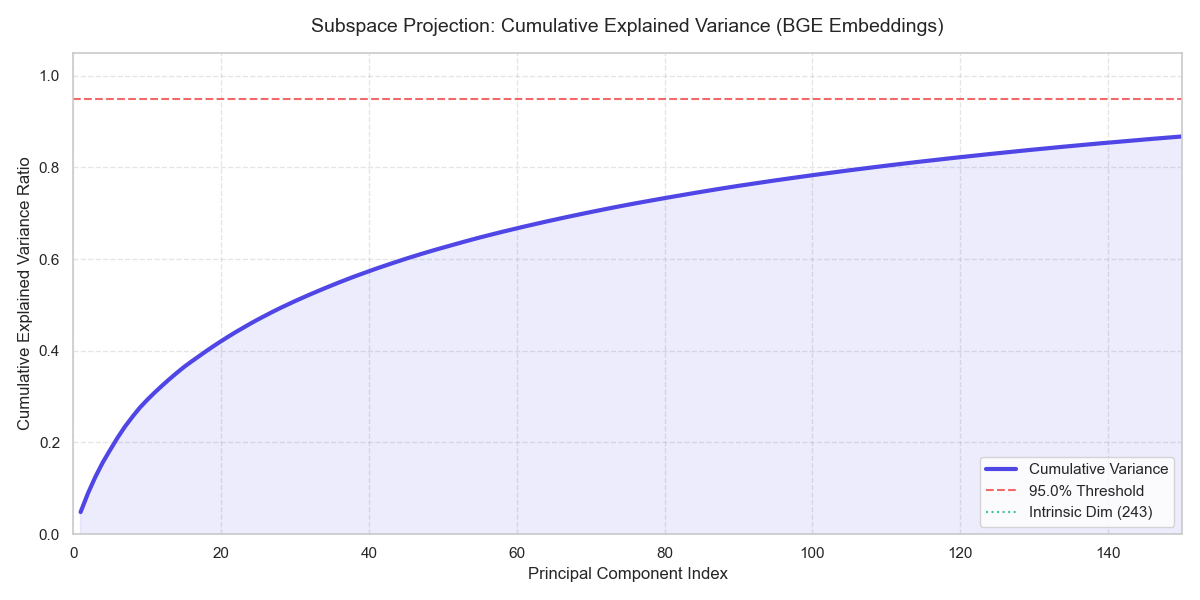
\includegraphics[width=\textwidth]{../variance_analysis_plot.png}
        \end{column}
    \end{columns}
\end{frame}
% SCRIPT FOR SLIDE 7:
% "Now that we know the 768-dimensional space contains redundancy and noise, how do we find a better coordinate system? We use Principal Component Analysis, or PCA.
%
% In linear algebra, we learn that a vector space can be represented using different bases. PCA is simply a change of basis. We are searching for a new orthonormal basis—meaning the basis vectors are all unit length and perpendicular to each other—that aligns with the shape of our data.
%
% The first new basis vector we choose points in the direction of the maximum variance, which is the direction of the greatest spread of our data points. Each subsequent basis vector we choose is orthogonal to the previous ones and captures the next largest spread.
%
% As you can see in the cumulative variance curve on the right, which is the actual plot generated from our live Pinecone production database, the curve climbs very steeply at first. This is because the first few basis vectors capture the main semantic patterns. The curve then flattens out, meaning additional dimensions are just adding tiny details and noise.
%
% By looking at this curve, we found that we can capture 90% of the total variance using only 220 dimensions instead of the original 768. This is a massive 71% reduction in dimensionality, which translates to a major boost in processing speed and storage savings in production."

% === Slide 8: PCA Variants & Information Loss ===
\begin{frame}{PCA Variants \& The Information Loss Trade-off}
    \textbf{Benchmarking 4 PCA Variants (384D Spider Dataset):}
    We run a timer to evaluate the speed, RAM efficiency, and accuracy trade-offs:

    \vspace{0.2cm}
    \begin{table}
        \centering
        \scriptsize
        \begin{tabular}{lp{2.4cm}p{3.8cm}}
            \hline
            \textbf{PCA Variant} & \textbf{RAM / Complexity} & \textbf{Trade-off \& Feature} \\ \hline
            \textbf{Standard} & Heavy on RAM & Loads all data; fastest and most accurate. \\
            \textbf{Incremental} & Very low RAM & Processes in mini-batches; nearly identical results. \\
            \textbf{Sparse} & Slowest & Forces weights to zero; highly interpretable. \\
            \textbf{Kernel} & High memory complexity & Maps to higher dimensions for curved patterns. \\ \hline
        \end{tabular}
    \end{table}

    \vspace{0.6cm}
    \textbf{Operational Verdict:}
    For query routing, standard PCA remains the baseline choice because of its high execution speed, while Incremental PCA provides the necessary memory scalability for large streaming databases.
\end{frame}
% SCRIPT FOR SLIDE 8:
% "While standard PCA is highly effective, we wanted to benchmark it against other variants to see how they handle memory constraints and data structures in a real-world pipeline. We conducted this benchmark on the 384-dimensional academic Spider dataset.
%
% First, standard PCA is our baseline. It is very fast and has the highest accuracy, but it requires loading the entire dataset into RAM at once. For massive enterprise scale, this is a memory bottleneck.
%
% To solve this, we tested Incremental PCA. Instead of loading all data, it processes the matrix in small, sequential chunks. We found that Incremental PCA consumes almost no RAM while yielding nearly identical coordinates to standard PCA.
%
% Next, we analyzed Sparse PCA. In standard PCA, every principal component is a linear combination of all 384 original dimensions, which makes them hard to interpret. Sparse PCA solves this by adding an L_1-regularization penalty, or Lasso penalty, on the component weights. This forces many weights to become exactly 0. The resulting principal components are composed of only a few key dimensions, making it highly interpretable for domain experts.
%
% Finally, we evaluated Kernel PCA. Standard PCA is a strictly linear transformation. Kernel PCA maps the data into a higher-dimensional space where curved, non-linear relationships become flat and linear. However, because it requires computing a kernel matrix—which means comparing every single query against every other query—its complexity scales quadratically. Our code had to restrict the run to 2,000 rows, which equates to 4 million comparisons, making it too slow for streaming production environments."

% === Slide 9: Results: Subspace and Blind Spots ===
\begin{frame}{Subspace Projection \& Geometric Blind Spots}
    \begin{columns}
        \begin{column}{0.46\textwidth}
            \textbf{Linear Subspace Projection (768D \(\rightarrow\) 2D):}
            \begin{itemize}
                \item We use a linear transformation to project the 768D space onto a 2D plane.
                \item \textbf{Analogy:} Shining a flashlight on a 768D object and observing its 2D shadow.
            \end{itemize}
            \vspace{0.15cm}
            \textbf{Key Geometric Insights:}
            \begin{itemize}
                \scriptsize
                \item \textbf{Easy Queries:} Tightly clustered (small distance variance), meaning they share highly repetitive linguistic structures.
                \item \textbf{Extra Hard Queries:} Geometrically dispersed (outliers), representing "blind spots."
            \end{itemize}
            \vspace{0.15cm}
            \textbf{Production Resolution:} Augmenting the database index with diverse nested-query examples to cover these blind spots.
        \end{column}
        
        \begin{column}{0.54\textwidth}
            \centering
            \textbf{\small 768D Embedding Space Projection}
            \vspace{0.1cm}
            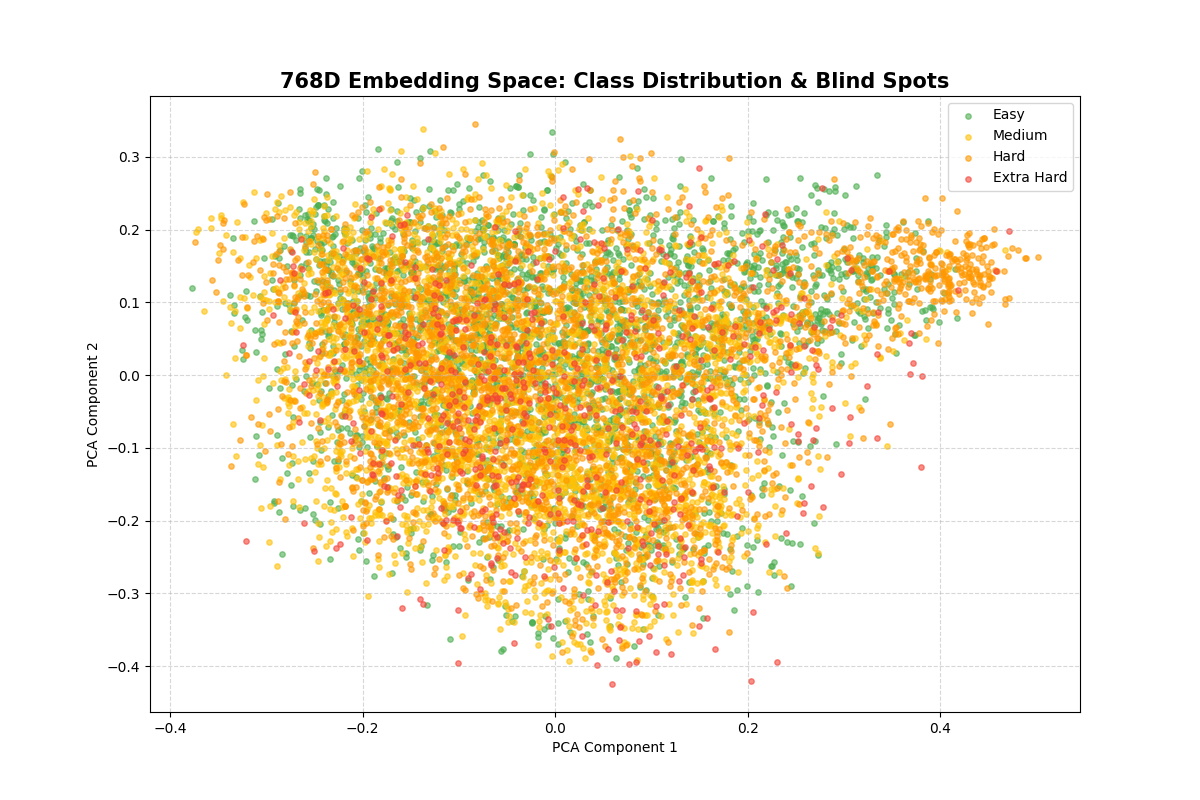
\includegraphics[width=1.06\textwidth]{../produc_vers/blind_spot_map.png}
        \end{column}
    \end{columns}
\end{frame}
% SCRIPT FOR SLIDE 9:
% "After choosing standard PCA as our dimensionality reduction tool, we wanted to look at the geometry of our embedding space. We project our 768-dimensional coordinates onto a 2D plane so we can inspect the distribution of our four complexity classes.
%
% Mathematically, we are applying a linear transformation to project a high-dimensional space down to two dimensions. The best way to visualize this is through a simple analogy: imagine shining a flashlight on a complex, 768-dimensional object. The plot we see on the right is the 2D shadow cast by that object on a flat wall.
%
% By examining this shadow, we uncovered crucial geometric insights about our data.
%
% First, if you look at the green points, which represent our 'Easy' queries, they are tightly clustered together. This means simple questions share highly repetitive semantic structures—they 'speak the same language' and lie in a very small pocket of the space.
%
% However, look at the orange points representing 'Extra Hard' queries. They do not form a cluster at all. Instead, they are widely dispersed across the outer boundaries of the space. These outliers are our 'blind spots.' They represent complex, rare SQL queries containing deep nests or unions that look completely different from one another.
%
% To resolve this in production, we cannot just hope the model learns these sparse regions. Instead, we use this geometric map to actively augment our database index with a wider, more diverse set of nested-query examples, filling in these blind spots.
%
% Now, seeing that our classes overlap and have curved boundaries in this 2D shadow, how do we draw boundary lines to separate them? This brings us to SVM classification and the Kernel Trick."

% === Slide 10: SVM Classification & The Kernel Trick ===
\begin{frame}{SVM Classification \& Kernel Benchmarks}
    \begin{columns}
        \begin{column}{0.55\textwidth}
            \textbf{Goal: Drawing Boundaries}
            We train a Support Vector Machine (SVM) to draw decision boundaries between query difficulty levels.
            
            \vspace{0.45cm}
            \textbf{Kernel Comparison (50 Components):}
            {\small
            \begin{itemize}
                \item \textbf{Linear Kernel (59.3\%):} Finds a straight boundary. Fails because class overlap is highly non-linear.
                \item \textbf{Polynomial Kernel (71.9\%):} Slower to execute (5.8s) and inconsistent on live production traffic.
                \item \textbf{RBF Kernel (73.4\%):} Chosen as our production standard. Fastest (3.8s) and most stable.
            \end{itemize}
            }
            \vspace{0.45cm}
            \textbf{Why RBF Works:} It uses a "local" approach that prioritizes nearby points, capturing tight "pockets" of Easy queries.
        \end{column}
        
        \begin{column}{0.45\textwidth}
            \centering
            \textbf{\small SVM Kernel Accuracies}
            \vspace{0.1cm}
            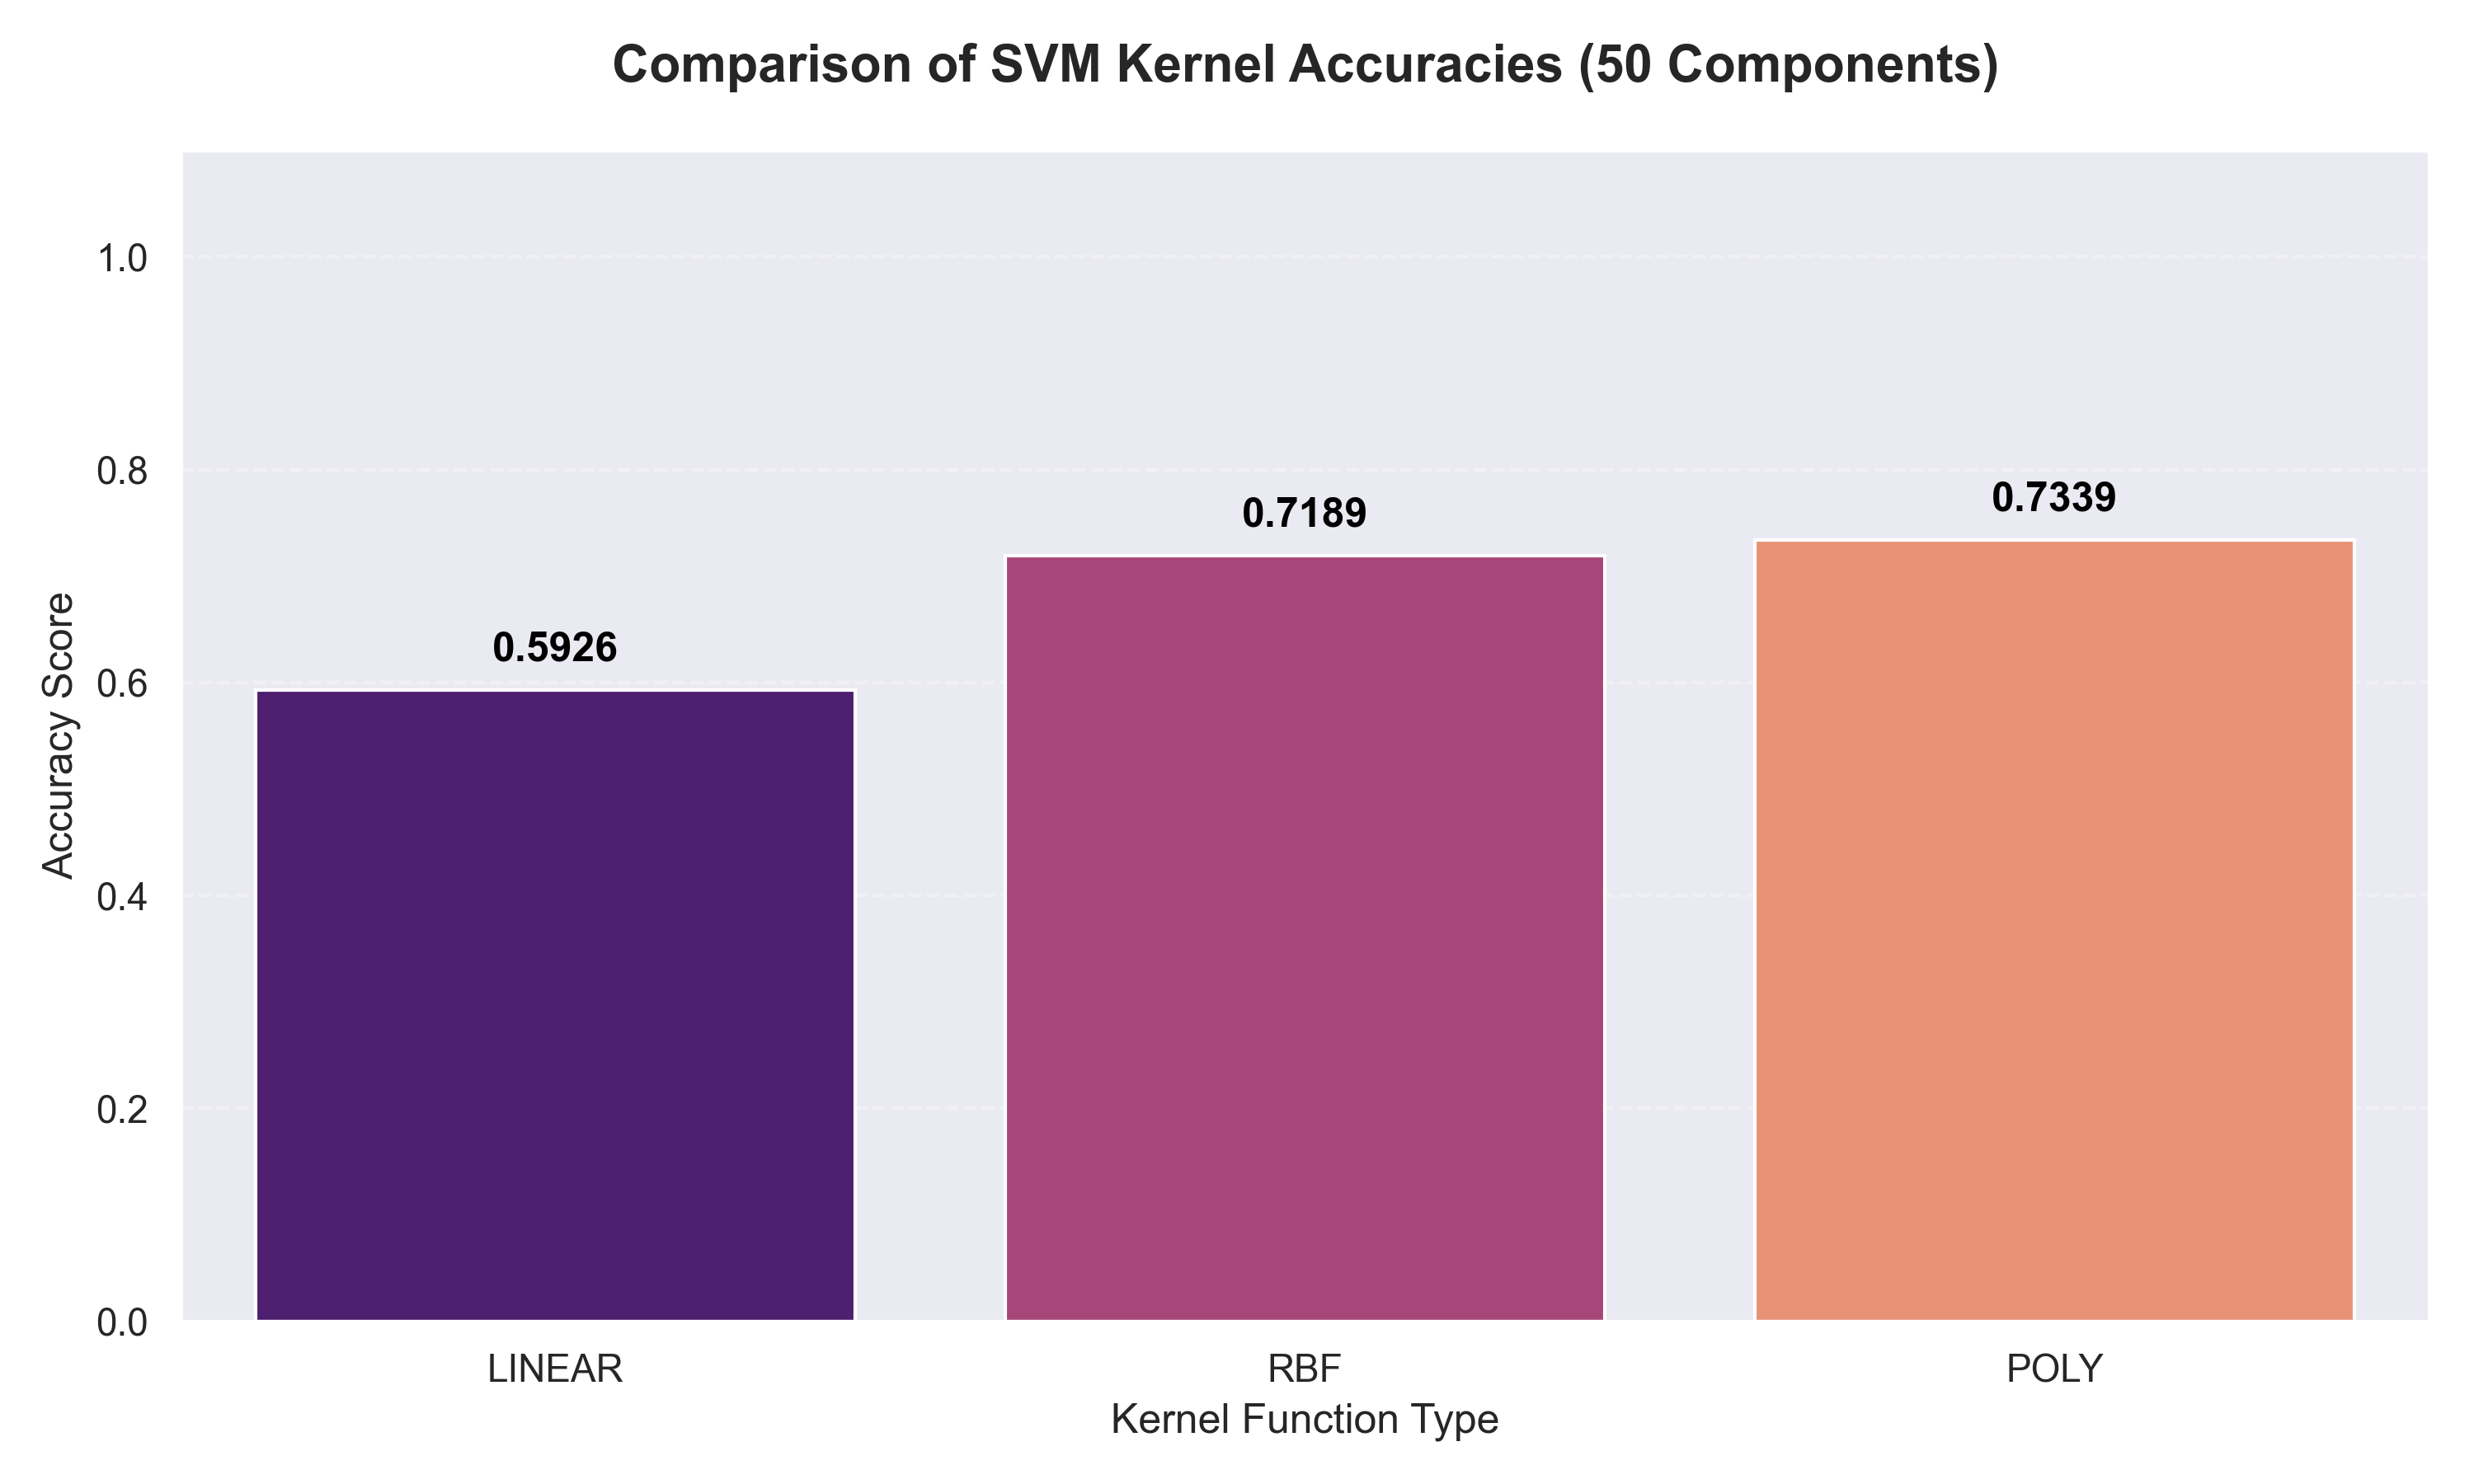
\includegraphics[width=\textwidth]{../phase4_kernel_comparison.png}
        \end{column}
    \end{columns}
\end{frame}
% SCRIPT FOR SLIDE 10:
% "Once we mapped our queries into the 220-dimensional subspace, our next task was building the classifier that routes them. We chose Support Vector Machines, or SVM, because they are mathematically designed to find the optimal boundary line that separates different classes of data.
%
% However, our queries are not perfectly separable by a straight line. If we try to use a standard Linear Kernel—which draws a flat boundary—the model fails, achieving a poor accuracy of only 59.3%. This is because the linguistic overlap between classes is too complex.
%
% To solve this, we use the Kernel Trick. The core idea is that if a dataset is not separable in its current space, we can map it to a higher-dimensional space where the curved boundaries become flat, allowing us to separate them cleanly.
%
% We benchmarked different types of kernels in Phase 4 of our research.
%
% First, the Polynomial Kernel captures curved boundaries, achieving a better accuracy of 71.9%. However, it is mathematically more complex to tune, takes longer to execute at nearly 6 seconds, and proved inconsistent when tested on live production traffic.
%
% Second, we tested the Radial Basis Function, or RBF kernel. RBF achieved our highest accuracy at 73.4% and was the fastest, executing in just 3.8 seconds. The mathematical secret behind RBF is that it uses a 'local' approach. It measures the exponential distance between points, meaning it prioritizes nearby queries. This is perfect for capturing the tight, dense 'pockets' of Easy queries we saw in our subspace projection.
%
% Having selected the RBF SVM as our routing engine, let's look at the final evaluation of our routing layer."

% === Slide 13: Model Evaluation and Routing ===
% === Slide 11: Results: Classification Performance ===
\begin{frame}{Results: Classification Performance}
    \begin{columns}[T]
        \begin{column}{0.46\textwidth}
            \textbf{Performance Evaluation:}
            \begin{table}
                \centering
                \scriptsize
                \begin{tabular}{lcc}
                    \hline
                    \textbf{Metric} & \textbf{384D (Spider)} & \textbf{768D (Production)} \\ \hline
                    SVM F1-Score & 0.71 & 0.81 \\
                    Routing Accuracy & 79\% & 89\% \\ \hline
                \end{tabular}
            \end{table}
            
            \vspace{0.2cm}
            \textbf{Key Insights:}
            \begin{itemize}
                \item \textbf{10-Point F1-Score Jump:} Moving from academic benchmarks to production vectors yields a massive boost.
                \item \textbf{Superior Separability:} Higher-dimensional production vectors ($\mathbb{R}^{768}$) spread out the semantic features, reducing linguistic overlap and allowing cleaner decision margins.
            \end{itemize}
        \end{column}
        
        \begin{column}{0.54\textwidth}
            \rule{0pt}{1.8cm}
            \centering
            \textbf{\small Separation: Spider vs. Live Platform}
            \vspace{-0.1cm}
            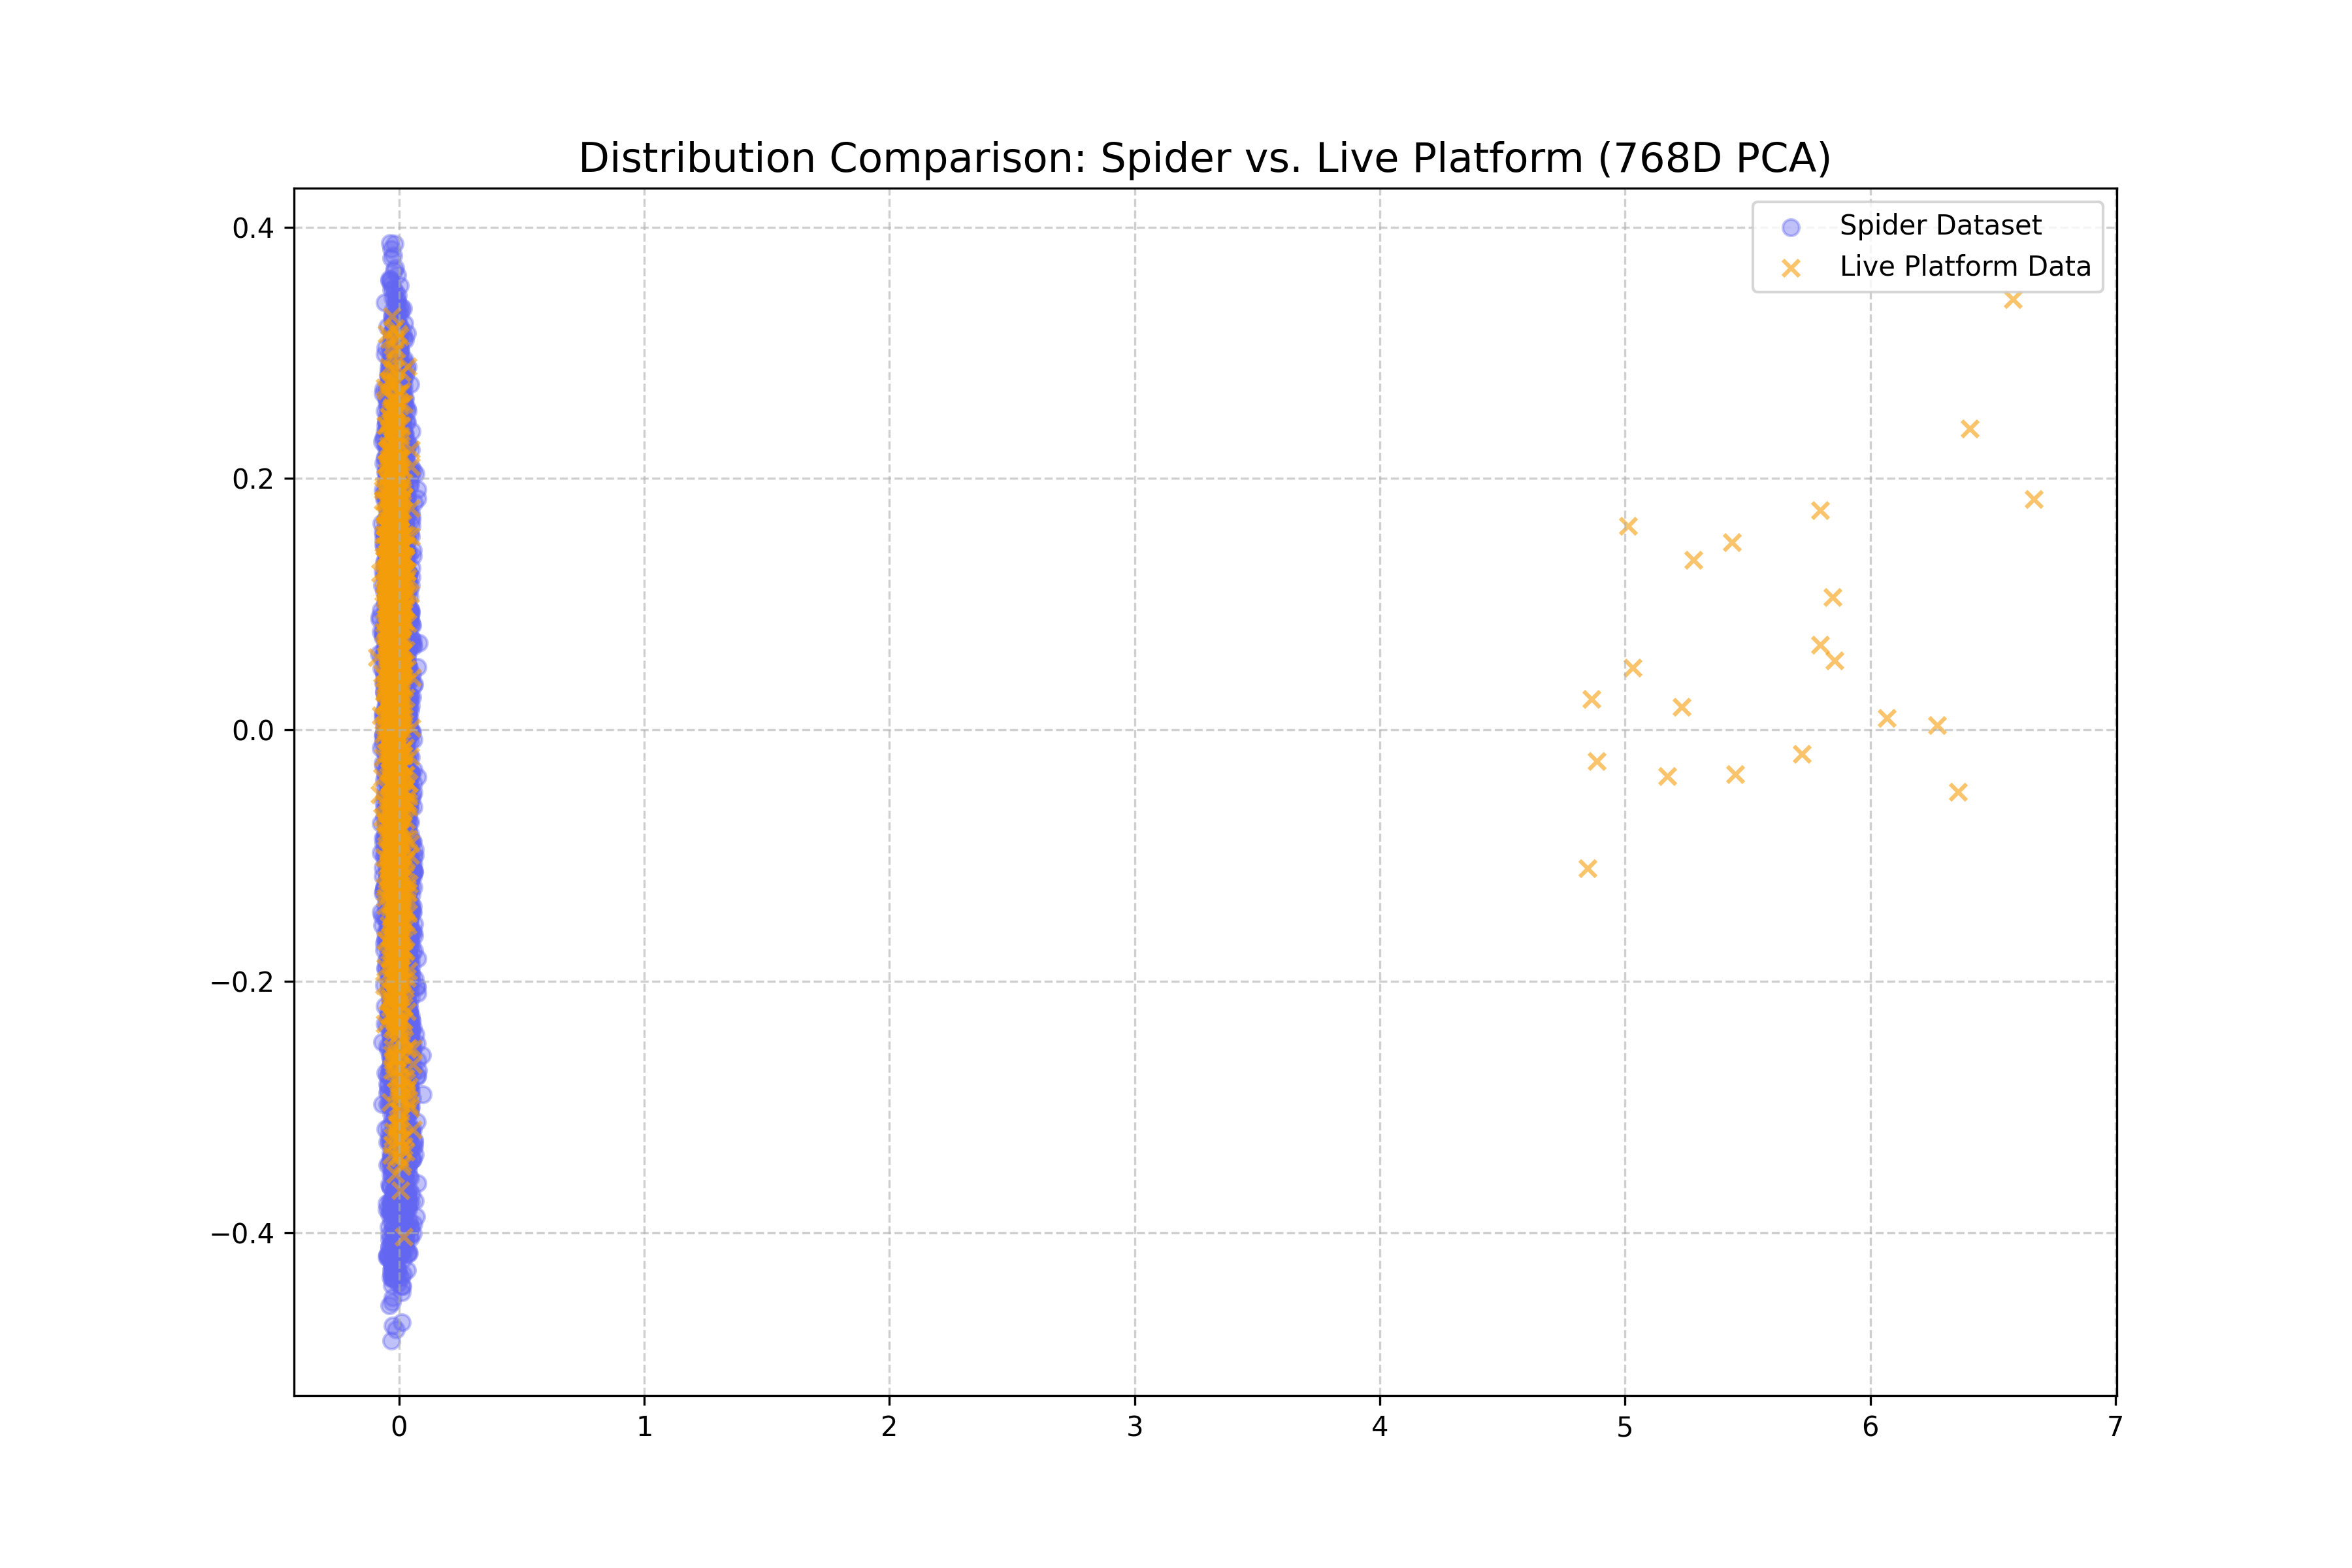
\includegraphics[width=0.95\textwidth]{../produc_vers/live_vs_spider_comparison.png}
        \end{column}
    \end{columns}
\end{frame}
% SCRIPT FOR SLIDE 11:
% "In Phase 5, we evaluate our final classifier's performance to see if it meets our production requirements.
%
% When we benchmarked our RBF SVM classifier on the academic Spider dataset in 384 dimensions, it achieved a respectable F1-score of 0.71. But when we migrated the exact same training pipeline to Sumvec's live 768-dimensional production vectors, our F1-score jumped by 10 points to 0.81.
%
% Let's look at the plot on the right to understand why this happens mathematically.
%
% The X-axis represents our sample counts, and the Y-axis is the relative semantic distance from the mean query. The blue points represent the academic Spider dataset, which are tightly compressed along a narrow band. The orange points represent our live production traffic, which spread out widely.
%
% Because the 768-dimensional space is larger, it allows the vector space embedding function to capture fine-grained semantic distinctions, reducing class overlap. Geometrically, this means the points are more spread out, giving our SVM a wider, cleaner margin to draw its decision boundaries.
%
% This performance validates that our classifier is highly reliable. Let's look at the actual business and infrastructure savings of this architecture in production."

% === Slide 12: Implications for Production Architecture ===
\begin{frame}{Implications for Production Architecture}
    \begin{columns}
        \begin{column}{0.5\textwidth}
            \textbf{Operational Verdict:}
            \begin{itemize}
                \item Standard PCA is the evidence-backed choice for Sumvec's database index.
                \item Eliminating the \textbf{71\% redundancy} yields faster similarity search and lower cloud costs.
            \end{itemize}
            
            \vspace{0.45cm}
            \textbf{Query Routing Rule:}
            \begin{itemize}
                \item \textbf{80\% of Traffic:} Rated Easy/Medium, routed to free models via Openrouter.
                \item \textbf{20\% of Traffic:} Rated Hard/Extra Hard, routed to Claude Haiku.
            \end{itemize}
        \end{column}
        
        \begin{column}{0.5\textwidth}
            \textbf{Production Cost Savings:}
            \vspace{0.2cm}
            \begin{table}
                \centering
                \scriptsize
                \begin{tabular}{lccc}
                    \hline
                    \textbf{Feature} & \textbf{Raw} & \textbf{PCA} & \textbf{Savings} \\ \hline
                    Dimensions & 768 & 220 & $\sim$ 71\% \\
                    Data Size & 37.2 MB & 10.9 MB & 26.3 MB \\ \hline
                \end{tabular}
            \end{table}
            
            \vspace{0.2cm}
            \begin{itemize}
                \scriptsize
                \item Reduces vector search latency.
                \item Lowers memory footprint on Pinecone.
                \item Meets our optimization constraint: $\text{Acc}(R(q)) \ge \alpha$.
            \end{itemize}
        \end{column}
    \end{columns}
\end{frame}
% SCRIPT FOR SLIDE 12:
% "To conclude, let's examine the real-world implications of our research on Sumvec's production architecture.
%
% First, our benchmark results prove that standard PCA is the optimal, evidence-backed choice for Pinecone vector compression. By compressing the database from 768 coordinates down to 220 coordinates, we eliminate 71% of redundant, noisy dimensions.
%
% As you can see in the table on the right, this compression reduces our active database footprint from 37.2 megabytes down to just 10.9 megabytes—saving over 26 megabytes. In cloud computing, this reduces the memory footprint on Pinecone, translating directly to lower infrastructure costs and faster similarity search lookups.
%
% Second, our routing layer is highly effective. The SVM classifier successfully identifies that 80% of our daily query traffic consists of Easy or Medium questions. The router directs these to free models from Openrouter, resolving them at zero inference cost. The remaining 20% of complex queries are directed to Claude Haiku, ensuring maximum accuracy for difficult requests.
%
% This realizes the optimization objective we stated at the very beginning of the presentation: minimizing cost and latency while keeping pipeline accuracy above our target threshold.
%
% Thank you, and I am happy to open the floor to any questions."

\end{document}
